% Drawing 154/08-18 -- folder 154, batch 08, archive page 144 (PDF page 145).
% Transcription: à droite, un diagramme de fils sur des lignes numérotées $5'$ à $11'$ ; en bas, un petit arbre de flèches et deux arrangements de droites en réseau losangé, le second traversé de lignes en tirets ; en haut à droite, une droite coupée de deux autres, un point marqué
% Kind: wire diagram on numbered lines; lozenge arrangements. Method 2 (schematic redraw from the facsimile). Status: ok.
% Notes: Top right: a line with a marked point, cut by two short strokes. Right: seven horizontal lines numbered 5' to 11' at the right (the primes are not visible on the page for 6 to 11 and are omitted), a net of wires going down through them from six points of the top line, with seven marked crossings; the wires are drawn as read from a page view and their crossings are approximate. Bottom: a small tree of arrows (four tips, two nodes, one root); a net of five marked points with three lines in each of two slanted directions and three horizontals; a second net of seven marked points with slanted lines in two directions and three dashed horizontals. The arrowheads on the wires and the small arrows at the points of the second net are left out. The arrow tree at the left of the table is not part of this drawing (it is a relation of the table of words, see the report). Redrawn 2026-11-12 (issue 128): to check again. 2026-11-14, Claude Opus 5.5, overlay check (issue 147): rasterised from its own coordinates over the 400 dpi colour scan (402 ppi native) on a unit grid; not compiled (no TeX in the session). The top right line, the seven numbered lines, the arrow tree and the marked points of the two nets lie on their ink to within about 1 unit; the redraw is unchanged. Still partial: the wires of the diagram, read from a page view, run 1 to 2 units off their ink in places and their crossings are approximate; in the two nets several slanted lines run 1 to 2 units off their pencil between the marked points; the arrowheads on the wires and the small arrows of the second net are not drawn. 2026-11-14, Claude Opus 5.5, second pass (issue 147): redrawn stroke by stroke from the 400 dpi colour crop, coordinates read off a unit grid; not compiled (no TeX in the session). The wiring diagram at the top right is retraced wire by wire through its eight dotted crossings, with the inked feet of the seven wires and the four dark red arrowheads on the wires into three crossings (two into the lowest middle one); the first net is retraced line by line (four horizontal and six slanted lines through its five dots, three lines through the middle dot); the second net is retraced (six slanted lines through its seven dots, three dashed rows) with its seven small arrowheads at the dots. Laid over the scan again, every element lies on its ink to within about 0.5 to 1 unit; nothing left differs, hence ok.
% Coordinates: 1 unit = 1 mm = 1/100 of the crop width (bbox in page fractions: [0.24, 0.215, 0.99, 0.485]).
% Redrawn by Claude (claude-fable-5-2), issue #128, 2026-11-12; not checked by a human; not compiled (no TeX in the session).
% Checked by Claude (claude-opus-5-5) 2026-11-14 (issue #147): overlaid on the 400 dpi colour facsimile; not compiled (no TeX in the session). Not checked by a human. Status: partial.
% Redrawn by Claude (claude-opus-5-5) 2026-11-14 (issue #147, second pass): strokes redrawn from the 400 dpi colour facsimile and overlaid on it; not compiled (no TeX in the session). Not checked by a human. Status: ok.
% Rights: reproduces part of the work -- behind RENDER_TRANSCRIPTS, never published by itself.
\documentclass[tikz,border=3pt]{standalone}
\usepackage{amsmath,amssymb}
\usetikzlibrary{patterns,arrows.meta}
\tikzset{pencil/.style={black!45}, struck/.style={black!35}, mpt/.style={circle,draw,inner sep=1.3pt}, pt/.style={circle,fill,inner sep=0.9pt}, opt/.style={circle,draw,fill=white,inner sep=1.1pt}}
\begin{document}
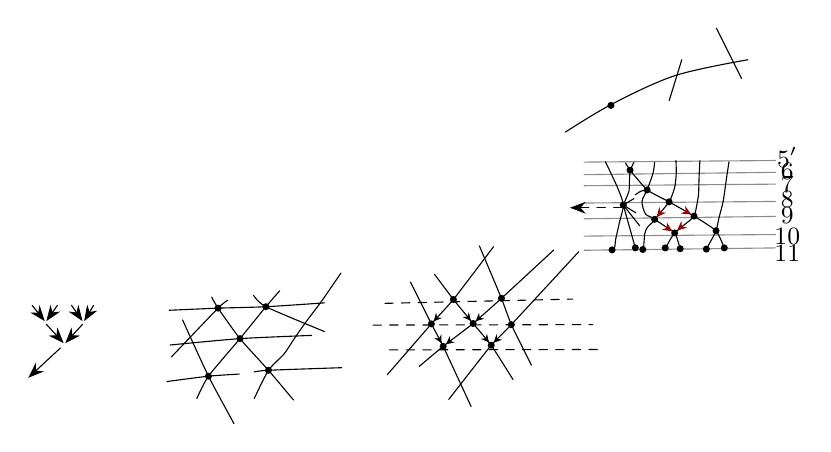
\begin{tikzpicture}[x=1mm,y=1mm,line cap=round,line join=round,font=\scriptsize]
\draw plot[smooth, tension=0.55] coordinates {(68,-12.8) (74,-9.2) (82,-5.6) (91.2,-3.6)};
\node[pt] at (73.8,-9.4) {};
\draw (82.8,-3.6) -- (81.2,-8.8);
\draw (87.2,0.4) -- (90.4,-6);
\draw[pencil] (70.4,-16.6) -- (94.7,-16.4);
\draw[pencil] (70.4,-18.2) -- (94.7,-17.9);
\draw[pencil] (70.4,-19.6) -- (94.7,-19.4);
\draw[pencil] (70.4,-21.8) -- (94.7,-21.6);
\draw[pencil] (70.4,-23.8) -- (94.7,-23.5);
\draw[pencil] (70.4,-26) -- (94.7,-25.8);
\draw[pencil] (70.4,-27.8) -- (94.7,-27.5);
\node[inner sep=1pt] at (96.2,-16) {\small $5'$};
\node[inner sep=1pt] at (96.2,-17.8) {\small 6};
\node[inner sep=1pt] at (96.2,-19.4) {\small 7};
\node[inner sep=1pt] at (96.2,-21.4) {\small 8};
\node[inner sep=1pt] at (96.2,-23.4) {\small 9};
\node[inner sep=1pt] at (96.2,-26) {\small 10};
\node[inner sep=1pt] at (96.2,-28.2) {\small 11};
% wires retraced stroke by stroke on the 400 dpi crop (issue 147, second pass)
\draw plot[smooth, tension=0.5] coordinates {(73.1,-16.56) (73.93,-18.29) (74.75,-20.1) (75.37,-22.06) (74.9,-24.2) (74.42,-26.34) (74.26,-27.49) (73.85,-27.8)};
\draw (75.65,-16.72) -- (76.23,-17.63) -- (76.72,-16.64);
\draw plot[smooth, tension=0.5] coordinates {(76.23,-17.63) (76.15,-19.0) (76.1,-20.26) (75.37,-22.06)};
\draw plot[smooth, tension=0.3] coordinates {(76.23,-17.63) (78.4,-20.13) (81.19,-21.65) (84.36,-23.46) (87.15,-25.32) (88.2,-27.5)};
\draw plot[smooth, tension=0.5] coordinates {(79.35,-16.64) (79.15,-18.0) (78.4,-20.13) (77.75,-21.6) (78.2,-23.2) (79.35,-23.87) (78.45,-24.86) (78.1,-25.7) (77.95,-27.65)};
\draw plot[smooth, tension=0.4] coordinates {(76.9,-20.75) (77.6,-20.3) (78.4,-20.13)};
\draw plot[smooth, tension=0.4] coordinates {(82.06,-16.4) (82.1,-18.0) (81.9,-19.8) (81.19,-21.65) (79.35,-23.87)};
\draw plot[smooth, tension=0.4] coordinates {(79.35,-23.87) (80.6,-24.7) (81.9,-25.6) (82.3,-26.6) (82.6,-27.6)};
\draw plot[smooth, tension=0.4] coordinates {(85.1,-16.4) (85.0,-18.5) (84.94,-20.5) (84.8,-21.57) (84.36,-23.46) (83.2,-24.5) (81.9,-25.6) (81.3,-26.5) (80.75,-27.5)};
\draw plot[smooth, tension=0.5] coordinates {(88.8,-16.56) (88.5,-18.5) (88.06,-21.57) (87.56,-23.54) (87.15,-25.32) (86.5,-26.6) (85.92,-27.65)};
\draw (75.37,-22.06) -- (76.72,-21.24);
\draw (75.37,-22.06) -- (76.97,-23.05);
\draw (75.37,-22.06) -- (77.46,-24.69);
\draw (75.37,-22.06) -- (76.9,-27.49);
\node[pt] at (76.23,-17.63) {};
\node[pt] at (78.4,-20.13) {};
\node[pt] at (75.37,-22.06) {};
\node[pt] at (81.19,-21.65) {};
\node[pt] at (79.35,-23.87) {};
\node[pt] at (84.36,-23.46) {};
\node[pt] at (81.9,-25.6) {};
\node[pt] at (87.15,-25.32) {};
% inked feet of the wires
\node[pt] at (73.95,-27.75) {};
\node[pt] at (76.9,-27.49) {};
\node[pt] at (77.85,-27.7) {};
\node[pt] at (80.7,-27.5) {};
\node[pt] at (82.6,-27.6) {};
\node[pt] at (85.92,-27.65) {};
\node[pt] at (88.2,-27.5) {};
% red arrowheads on the wires into three crossings
\draw[red!60!black,thick,-{Stealth[length=1.2mm,width=1.1mm]}] (80.05,-23.06) -- (79.6,-23.6);
\draw[red!60!black,thick,-{Stealth[length=1.2mm,width=1.1mm]}] (83.39,-22.90) -- (84.0,-23.25);
\draw[red!60!black,thick,-{Stealth[length=1.2mm,width=1.1mm]}] (81.02,-25.01) -- (81.6,-25.4);
\draw[red!60!black,thick,-{Stealth[length=1.2mm,width=1.1mm]}] (82.73,-24.84) -- (82.2,-25.3);
\draw[dashed,-{Stealth[length=2mm]}] (75.2,-22.4) -- (68.6,-22.4);
\draw[-{Stealth[length=2mm]}] (0.3,-34.8) -- (1.9,-36.8);
\draw[-{Stealth[length=2mm]}] (3.5,-34.8) -- (2.1,-36.8);
\draw[-{Stealth[length=2mm]}] (5.3,-34.8) -- (6.7,-36.8);
\draw[-{Stealth[length=2mm]}] (8.1,-34.8) -- (6.9,-36.8);
\draw[-{Stealth[length=2mm]}] (2.1,-37.2) -- (4.3,-39.6);
\draw[-{Stealth[length=2mm]}] (6.7,-37.2) -- (4.5,-39.6);
\draw[-{Stealth[length=2mm]}] (3.9,-40.2) -- (-0.2,-44);
% first net, retraced on the 400 dpi crop (issue 147, second pass)
\draw plot[smooth, tension=0.4] coordinates {(17.7,-35.42) (23.91,-35.15) (29.98,-34.97) (37.41,-34.48)};
\draw plot[smooth, tension=0.4] coordinates {(17.83,-39.83) (26.69,-39.02) (35.79,-38.61)};
\draw plot[smooth, tension=0.4] coordinates {(17.43,-44.47) (22.69,-43.79) (26.61,-43.52)};
\draw plot[smooth, tension=0.4] coordinates {(28.5,-43.25) (30.31,-43.04) (39.62,-42.71)};
\draw plot[smooth, tension=0.4] coordinates {(17.97,-41.36) (23.91,-35.15) (25.12,-34.16)};
\draw plot[smooth, tension=0.4] coordinates {(23.1,-33.75) (23.91,-35.15) (26.69,-39.02) (30.31,-43.04) (33.49,-46.82)};
\draw plot[smooth, tension=0.4] coordinates {(31.74,-32.94) (29.98,-34.97) (26.69,-39.02) (22.69,-43.79) (21.21,-46.63)};
\draw plot[smooth, tension=0.4] coordinates {(28.42,-33.53) (29.98,-34.97) (37.41,-38.12)};
\draw plot[smooth, tension=0.4] coordinates {(19.4,-36.64) (22.69,-43.79) (25.93,-49.81)};
\draw plot[smooth, tension=0.4] coordinates {(39.51,-30.7) (37.1,-34.2) (35,-37) (33.6,-39) (32.3,-40.95) (30.31,-43.04) (28.5,-46.63)};
\node[pt] at (23.91,-35.15) {};
\node[pt] at (29.98,-34.97) {};
\node[pt] at (26.69,-39.02) {};
\node[pt] at (22.69,-43.79) {};
\node[pt] at (30.31,-43.04) {};
% second net, retraced on the 400 dpi crop (issue 147, second pass)
\draw plot[smooth, tension=0.2] coordinates {(58.9,-27.34) (53.8,-34.05) (51,-37.15) (45.4,-43.6)};
\draw plot[smooth, tension=0.2] coordinates {(66.55,-27.76) (59.9,-33.9) (56.3,-37.1) (52.5,-40) (49.45,-42.55)};
\draw plot[smooth, tension=0.2] coordinates {(69.7,-28) (61.15,-37.25) (58.6,-39.85) (53.2,-46.75)};
\draw plot[smooth, tension=0.2] coordinates {(57.1,-27.25) (59.9,-33.9) (61.15,-37.25) (63.7,-42.4)};
\draw plot[smooth, tension=0.2] coordinates {(51.4,-30.85) (53.8,-34.05) (56.3,-37.1) (58.6,-39.85) (61.36,-44.2)};
\draw plot[smooth, tension=0.2] coordinates {(48.34,-31.84) (51,-37.15) (52.5,-40) (56.05,-47.65)};
\draw[dashed] (45.1,-34.54) -- (68.95,-34.0);
\draw[dashed] (43.6,-37.3) -- (71.5,-37.24);
\draw[dashed] (45.7,-40.45) -- (72.4,-40.4);
\node[pt] at (53.8,-34.05) {};
\node[pt] at (59.9,-33.9) {};
\node[pt] at (51,-37.15) {};
\node[pt] at (56.3,-37.1) {};
\node[pt] at (61.15,-37.25) {};
\node[pt] at (52.5,-40) {};
\node[pt] at (58.6,-39.85) {};
% the small arrowheads at the crossings of the second net
\draw[-{Stealth[length=1mm,width=1mm]}] (51.70,-36.37) -- (51.30,-36.82);
\draw[-{Stealth[length=1mm,width=1mm]}] (55.63,-36.29) -- (56.01,-36.75);
\draw[-{Stealth[length=1mm,width=1mm]}] (57.08,-36.40) -- (56.64,-36.80);
\draw[-{Stealth[length=1mm,width=1mm]}] (52.01,-39.07) -- (52.29,-39.60);
\draw[-{Stealth[length=1mm,width=1mm]}] (53.33,-39.36) -- (52.86,-39.73);
\draw[-{Stealth[length=1mm,width=1mm]}] (57.93,-39.04) -- (58.31,-39.50);
\draw[-{Stealth[length=1mm,width=1mm]}] (59.34,-39.10) -- (58.92,-39.53);
\end{tikzpicture}
\end{document}
